\section{Evaluating the Full Family of DINOv3 Models}
\label{sec:family}
In this section, we provide quantitative evaluations on the family of models distilled from our 7B-parameters model (See \cref{sec:distillation}). 
This family includes variants based on the Vision Transformer (ViT) and the ConvNeXt (CNX) architectures.
We provide the detailed parameter counts and inference FLOPs for all models in \cref{tab:family-models-flops}. 
These models cover a wide range of computational budgets to accommodate a broad spectrum of users and deployment scenarios. 
We conduct a thorough evaluation of all ViT (\cref{sec:family:vits}) and ConvNeXt variants to assess their performance across tasks.

\Cref{fig:intro:family} provides an overview comparison of the DINOv3 family versus other model collections.
The DINOv3 family significantly outperforms all others on dense prediction tasks.
This includes specialized models distilled from supervised backbones like AM-RADIO and PEspatial.
At the same time, our models achieve similar results on classification tasks, making them the optimal choice across compute budgets.

In \cref{sec:family:vits} detail our ViT models and compare them to other open-source alternatives.
Then, in \cref{sec:family:convnext}, we discuss the ConvNeXt models.
Finally, following \cref{sec:alignementtxt}, we trained a text encoder aligned with the output of our ViT-L model.
We present multi-modal alignment results for this model in \cref{sec:family:text}. 



\begin{figure}[t]
    \centering
    \begin{subfigure}[b]{0.5\textwidth}
        \centering
        \begin{tabular}{l r rr}
            \toprule
             &  & \multicolumn{2}{c}{Inference GFLOPs} \\
             \cmidrule{3-4}
            Model & \#Params & Res.~256 & Res.~512 \\
             \midrule
            CNX-Tiny & 29M & 5 & 20  \\
            CNX-Small & 50M & 11 & 46 \\
            CNX-Base & 89M  & 20 & 81 \\
            CNX-Large & 198M & 38 & 152  \\
             \midrule
            ViT-S &  21M & 12 & 63 \\
            ViT-S+ & 29M & 16 & 79 \\
            ViT-B &  86M  & 47 & 216 \\
            ViT-L &  300M & 163 & 721 \\
            ViT-H+ & 840M  & 450 & 1903 \\
             \midrule
            ViT-7B & 6716M & 3550 & 14515 \\
            \bottomrule
        \end{tabular}
        \caption{DINOv3 family of models.}
        \label{tab:family-models-flops}
    \end{subfigure}
    \hfill
    \begin{subfigure}[b]{0.48\textwidth}    
        \centering 
        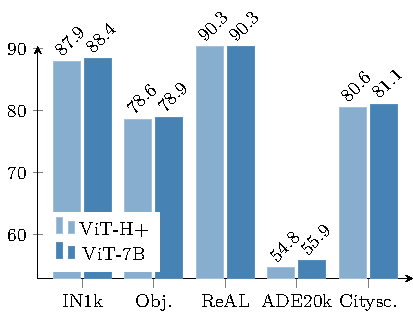
\includegraphics{figures/tikz/family_h_vs_7b.pdf} 
        \caption{ViT-H+ v.s. ViT-7B.}
        \label{fig:family:vith-7b}
    \end{subfigure}
    \caption{
        (a) Presentation of the distilled models' characteristics. 
        CNX stands for ConvNeXT. We present per model the number of parameters and the GFLOPs estimated on images of size $256\times256$ and $512\times512$. 
        (b) We compare DINOv3 ViT-H+ to its 7B-sized teacher; despite having almost 10$\times$ less parameters, the ViT-H+ is close to DINOv3 7B in performance.
    }
\end{figure}


\subsection{A Vision Transformer for Every Use Case}
\label{sec:family:vits}
Our ViT family spans architectures from the compact ViT-S to the larger 840 million parameter ViT-H+ models.
The former is designed to run efficiently on resource-constrained devices such as laptops, the latter delivers state-of-the-art performance for more demanding applications.
We compare our ViT models to the best open-source image encoders of corresponding size, namely DINOv2~\citep{oquab2024dinov2}, SigLIP~2~\citep{tschannen2025siglip} and Perception Encoder~\citep{bolya2025perception}. 
For a fair comparison, we ensure that the input sequence length is equivalent across models. 
Specifically, for model with a patch size of 16 we input images of size $512 \times 512$ versus $448 \times 448$ when models are using patch size 14. 

\begin{table}[t]
  \centering
  \small
  \caption{
    Comparison of our family of models against open-source alternatives of comparable size.
    We showcase our ViT-\{S, S+, B, L, H+\} models on a representative set of global and dense benchmarks: classification (IN-ReAL, IN-R, ObjectNet), retrieval (Oxford-H), segmentation (ADE20k), depth (NYU), tracking (DAVIS at 960px), and keypoint matching (NAVI, SPair).
    We match the number of patch tokens for a fair comparison across models of different patch size.
  }
  \label{tab:family:distillation}
  \begin{tabular}{@{}llc cccc c ccccc@{}}
    \toprule
    & && \multicolumn{4}{c}{Global Tasks} && \multicolumn{5}{c}{Dense Tasks} \\
    \cmidrule{4-7} \cmidrule{9-13}
    Size & Model && IN-ReaL & IN-R & Obj. & Ox.-H && ADE20k  & NYU$\downarrow$ & DAVIS & NAVI & SPair \\
    \midrule
    S & DINOv2  && 87.3 & 54.0 & 47.8 & 39.5 && 45.5 & 0.446 & 73.6 & 53.4 & 51.6 \\
    S & DINOv3  && 87.0 & 60.4 & 50.9 & 49.5 && 47.0 & 0.403 & 72.7 & 56.3 & 50.4 \\
    S+ & DINOv3 && 88.0 & 68.8 & 54.6 & 50.0 && 48.8 & 0.399 & 75.5 & 57.1 & 55.2 \\  
    \midrule
    B & PEcore && 87.5 & 68.4 & 57.9 & 20.2 && 37.4 & 0.641 & 44.5 & 41.8 & 13.7 \\ 
    B & SigLIP 2 && 89.3 & 80.6 & 66.9 & 20.2 && 41.6 & 0.512 & 63.2 & 45.4 & 32.8\\
    B & DINOv2  && 89.0 & 68.4 & 57.3 & 51.0 && 48.4 & 0.416 & 72.9 & 56.9 & 57.1 \\
    B & DINOv3  && 89.3 & 76.7 & 64.1 & 58.5 && 51.8 & 0.373 & 77.2 & 58.8 & 57.2 \\ 
    \midrule
    L & PEcore && 90.1 & 87.7 & 74.9 & 25.6 && 39.7 & 0.650 & 48.2 & 42.1 & 19.2 \\
    L & SigLIP 2 && 90.1 & 89.2 & 75.0 & 21.4 && 43.6 & 0.484 & 66.3 & 47.8 & 41.9 \\
    L & DINOv2  && 89.7 & 79.1 & 64.7 & 55.7 && 48.8 & 0.394 & 73.4 & 59.9 & 57.0 \\
    L & DINOv3  && 90.2 & 88.1 & 74.8 & 63.1 && 54.9 & 0.352 & 79.9 & 62.3 & 61.2 \\
    \midrule
    SO400m & SigLIP 2 && 90.3 & 90.4 & 76.2 & 23.0 && 44.0 & 0.402 & 64.8 & 48.8 & 38.7 \\
    \midrule
    H+ & DINOv3 && 90.3 & 90.0 & 78.6 & 64.5 && 54.8 & 0.352 & 79.3 & 63.3 & 56.3 \\ 
    \bottomrule
  \end{tabular}
\end{table}

Our empirical study clearly demonstrates that DINOv3 models consistently outperform their counterparts on dense prediction tasks. 
Most notably, on the ADE20k benchmark, the DINOv3 ViT-L model achieves an improvement of over 6 mIoU points compared to the best competitor DINOv2.
The ViT-B variant shows a gain of approximately 3 mIoU points against the next best competitor. 
These substantial improvements highlight the effectiveness of DINOv3's local features in capturing fine-grained spatial details. 
Furthermore, evaluations on depth estimation tasks also reveal consistent performance gains over competing approaches.
This underscores the versatility of the DINOv3 family across different dense vision problems. 
Importantly, our models achieve competitive results on global recognition benchmarks such as ObjectNet and ImageNet-1k.
This indicates that the enhanced dense task performance does not come at the expense of global task accuracy. 
This balance confirms that DINOv3 models provide a robust and well-rounded solution, excelling across both dense and global vision tasks without compromise.

On another note, we want to also validate if the largest models that we distill capture all the information from the teacher.
To this end, we run a comparison of our largest ViT-H+ with the 7B teacher.
As shown in \cref{fig:family:vith-7b}, the largest student achieves performance that is on par with the 8 times larger ViT-7B model. 
This result not only validates the effectiveness of our distillation process but also demonstrates that, when guided by a high-quality teacher, smaller models can learn to deliver comparable levels of performance. 
This finding reinforces our belief that \emph{training very large models benefits the broader community}.
The strength of larger models can be successfully distilled into more efficient, smaller models with little or no loss of quality.

\begin{figure}[t]
    \centering
    \begin{tikzpicture}[every node/.style={inner sep=0, outer sep=0}]
        \newcommand{\imgHSpace}{0.15cm} %
        \newcommand{\imgVSpace}{0.15cm} %
        \newcommand{\imgSize}{0.21\textwidth}
        \node (img11) {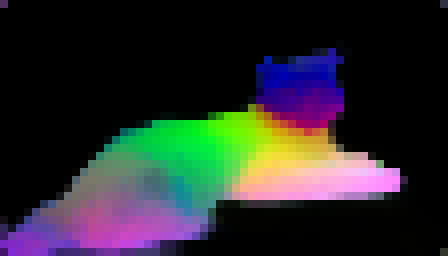
\includegraphics[width=\imgSize]{figures/analysis/family_resolutions/vits512_cat_marc_pca_rgb.png}};
        \node[right=\imgHSpace of img11] (img12) {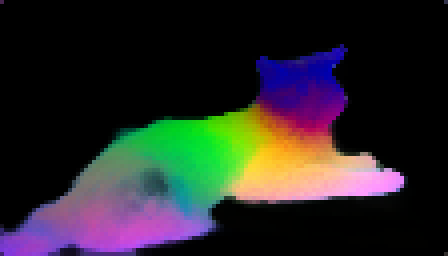
\includegraphics[width=\imgSize]{figures/analysis/family_resolutions/vits1024_cat_marc_pca_rgb.png}};
        \node[right=\imgHSpace of img12] (img13) {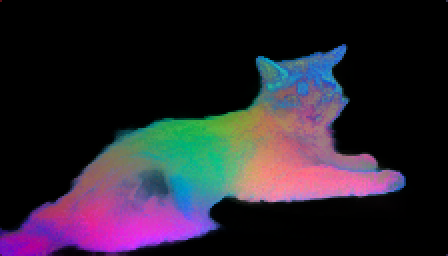
\includegraphics[width=\imgSize]{figures/analysis/family_resolutions/vits2048_cat_marc_pca_rgb.png}};
        \node[right=\imgHSpace of img13] (img14) {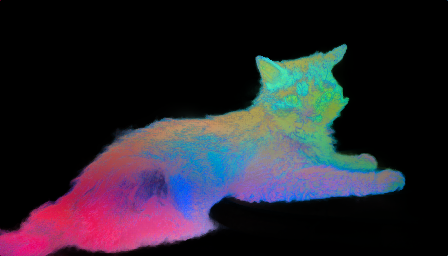
\includegraphics[width=\imgSize]{figures/analysis/family_resolutions/vits4096_cat_marc_pca_rgb.png}};
        \node[below=\imgVSpace of img11] (img21) {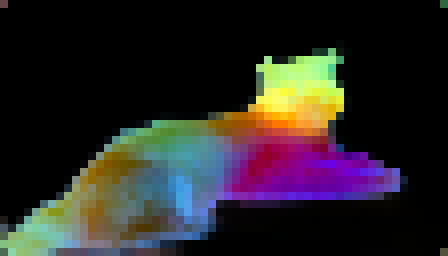
\includegraphics[width=\imgSize]{figures/analysis/family_resolutions/vitsp512_cat_marc_pca_rgb.png}};
        \node[right=\imgHSpace of img21] (img22) {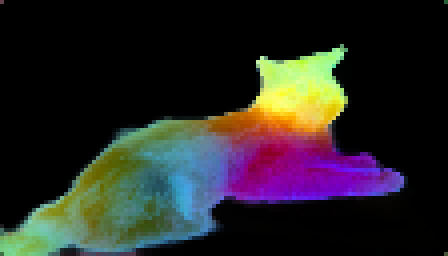
\includegraphics[width=\imgSize]{figures/analysis/family_resolutions/vitsp1024_cat_marc_pca_rgb.png}};
        \node[right=\imgHSpace of img22] (img23) {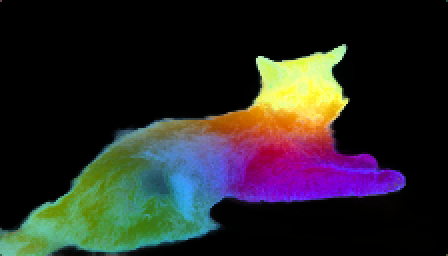
\includegraphics[width=\imgSize]{figures/analysis/family_resolutions/vitsp2048_cat_marc_pca_rgb.png}};
        \node[right=\imgHSpace of img23] (img24) {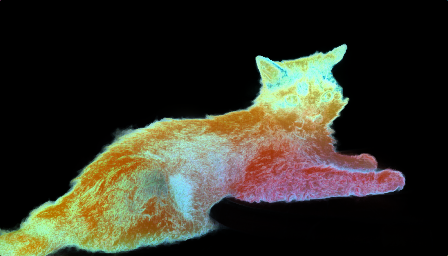
\includegraphics[width=\imgSize]{figures/analysis/family_resolutions/vitsp4096_cat_marc_pca_rgb.png}};
        \node[below=\imgVSpace of img21] (img31) {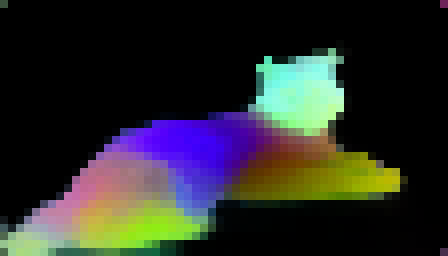
\includegraphics[width=\imgSize]{figures/analysis/family_resolutions/vitb512_cat_marc_pca_rgb.png}};
        \node[right=\imgHSpace of img31] (img32) {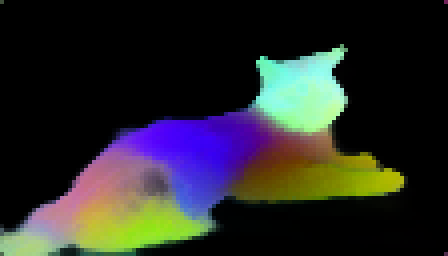
\includegraphics[width=\imgSize]{figures/analysis/family_resolutions/vitb1024_cat_marc_pca_rgb.png}};
        \node[right=\imgHSpace of img32] (img33) {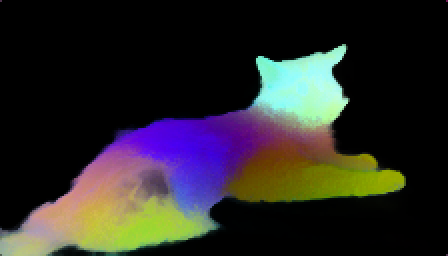
\includegraphics[width=\imgSize]{figures/analysis/family_resolutions/vitb2048_cat_marc_pca_rgb.png}};
        \node[right=\imgHSpace of img33] (img34) {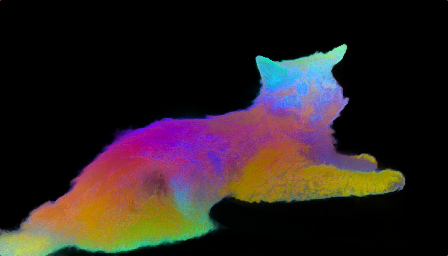
\includegraphics[width=\imgSize]{figures/analysis/family_resolutions/vitb4096_cat_marc_pca_rgb.png}};
        \node[below=\imgVSpace of img31] (img41) {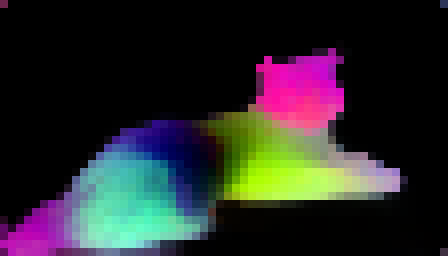
\includegraphics[width=\imgSize]{figures/analysis/family_resolutions/vitl512_cat_marc_pca_rgb.png}};
        \node[right=\imgHSpace of img41] (img42) {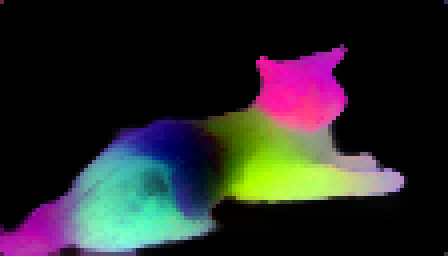
\includegraphics[width=\imgSize]{figures/analysis/family_resolutions/vitl1024_cat_marc_pca_rgb.png}};
        \node[right=\imgHSpace of img42] (img43) {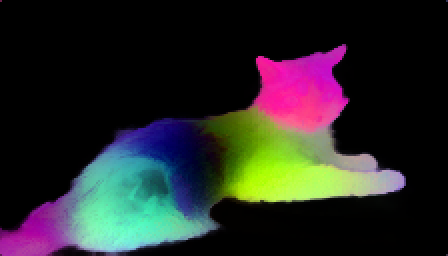
\includegraphics[width=\imgSize]{figures/analysis/family_resolutions/vitl2048_cat_marc_pca_rgb.png}};
        \node[right=\imgHSpace of img43] (img44) {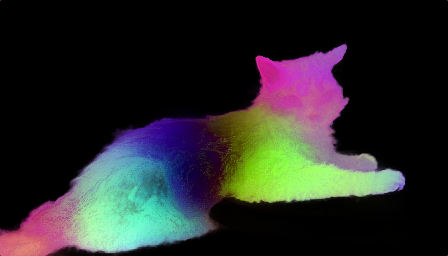
\includegraphics[width=\imgSize]{figures/analysis/family_resolutions/vitl4096_cat_marc_pca_rgb.png}};
        \node[below=\imgVSpace of img41] (img51) {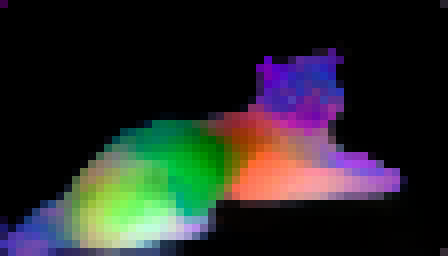
\includegraphics[width=\imgSize]{figures/analysis/family_resolutions/vith512_cat_marc_pca_rgb.png}};
        \node[right=\imgHSpace of img51] (img52) {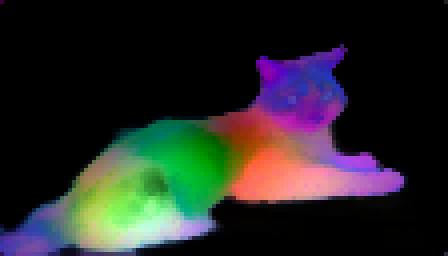
\includegraphics[width=\imgSize]{figures/analysis/family_resolutions/vith1024_cat_marc_pca_rgb.png}};
        \node[right=\imgHSpace of img52] (img53) {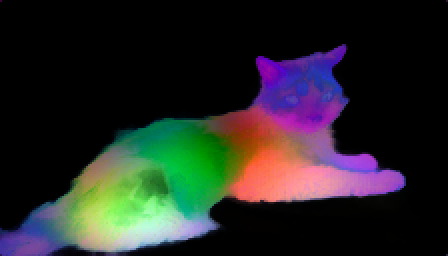
\includegraphics[width=\imgSize]{figures/analysis/family_resolutions/vith2048_cat_marc_pca_rgb.png}};
        \node[right=\imgHSpace of img53] (img54) {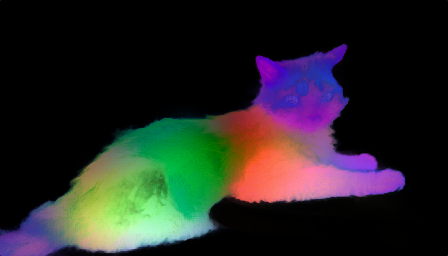
\includegraphics[width=\imgSize]{figures/analysis/family_resolutions/vith4096_cat_marc_pca_rgb.png}};
        \node[anchor=center] (label1) [left=0.3cm of img11.west] {\rotatebox{90}{ViT-S}};
        \node[anchor=center] (label2) [left=0.3cm of img21.west] {\rotatebox{90}{ViT-S+}};
        \node[anchor=center] (label3) [left=0.3cm of img31.west] {\rotatebox{90}{ViT-B}};
        \node[anchor=center] (label4) [left=0.3cm of img41.west] {\rotatebox{90}{ViT-L}};
        \node[anchor=center] (label5) [left=0.3cm of img51.west] {\rotatebox{90}{ViT-H+}};
        \node[below=0.2cm of img51.south] {\small $896\times512$};
        \node[below=0.2cm of img52.south] {\small $1792\times1024$};
        \node[below=0.2cm of img53.south] {\small $3584\times2048$};
        \node[below=0.2cm of img54.south] {\small $7168\times4096$};
    \end{tikzpicture}
    \caption{Stability of the features at multiple resolutions for the DINOv3 ViT family of models. 
    Top-to-bottom: ViT-S, S+, B, L, H+. 
    We run inference on an image at multiple resolutions, then perform principal component analysis on the features computed on a $1792\times1024$ image ($112\times64$ image tokens).
    We then project features at all resolutions onto the principal components 5--7 that we map to the RGB space for visualization. 
    While the models are functional at all resolutions, we observe that the features remain consistent across a large range of resolutions before drifting: for example, ViT-S+ features are stable between $896\times512$ and $3584\times2048$ inputs, while ViT-L barely starts drifting on the largest resolution $7168\times4096$. 
    ViT-H+ remains stable throughout the whole tested range.}
    \label{fig:pca:family}
\end{figure}


    
    



\subsection{Efficient ConvNeXts for Resource-Constrained Environments}
\label{sec:family:convnext}

In this section, we evaluate the quality of our ConvNeXt (CNX) models distilled from the 7B teacher. 
ConvNeXt models are highly efficient in terms of FLOPs and are well-suited for deployment on devices optimized for convolutional computations. 
Furthermore, transformer models often do not lend themselves well to quantization~\citep{bondarenko2021understanding}, whereas quantization of convolutional nets is a well explored subject.
We distill CNX architectures of size T, S, B, and L (see \cref{tab:family-models-flops}) and compare them to the original ConvNeXt models~\citep{liu2022convnet}.
These baselines achieve high performance on ImageNet-1k as they were trained in a supervised fashion using ImageNet-22k labels, and thus represent a strong competitor.
For this experiment, we provide results for global tasks at input resolutions 256 and 512, for ADE20k at resolution 512, and for NYU at resolution 640.

\begin{table}[t]
    \centering
    \caption{
      Evaluation of our distilled DINOv3 ConvNeXt models.
      We compare our models to off-the-shelf ConvNeXts trained supervised on ImageNet-22k~\citep{liu2022convnet}.
      For global tasks, we give results at input resolutions 256 and 512, as we found the supervised models to significantly degrade at resolution 512.
    }
    \begin{tabular}{@{}ll c  cc c cc c cc  c cc@{}}
    \toprule
    & && \multicolumn{8}{c}{Global Tasks} && \multicolumn{2}{c}{Dense Tasks} \\
    \cmidrule{4-11} \cmidrule{13-14}
    Size & Model && \multicolumn{2}{c}{IN-ReAL} && \multicolumn{2}{c}{IN-R} && \multicolumn{2}{c}{Obj.} && ADE20k & NYU$\downarrow$ \\
    \cmidrule{4-5} \cmidrule{7-8} \cmidrule{10-11}
    &&& 256 & 512 && 256 & 512 && 256 & 512 && & \\
    \midrule
    T & Sup.  && 87.3 & 83.0 && 45.0 & 33.0 && 44.5 & 27.1 && 24.8 & 0.666 \\
    T & DINOv3 && 86.6 & 87.7 && 73.7 & 74.1 && 52.6 & 58.7 && 42.7 & 0.448 \\
    \midrule
    S & Sup.  && 88.9 & 86.8 && 52.8 & 39.1 && 50.8 & 40.0 && 22.6 & 0.630 \\
    S & DINOv3  && 87.9 & 88.7 && 73.7 & 74.1 && 52.6 & 58.7 && 44.8 & 0.432\\
    \midrule
    B & Sup.  && 89.3 & 87.8 && 57.3 & 46.2 && 53.6 & 46.5 && 26.5 & 0.596 \\
    B & DINOv3  && 88.5 & 89.2 && 77.2 & 78.2 && 56.2 & 61.3 && 46.3 & 0.420 \\
    \midrule
    L & Sup.  && 89.6 & 88.1 && 58.4 & 46.6 && 55.0 & 47.7 && 33.3 & 0.567 \\
    L & DINOv3  && 88.9 & 89.4 && 81.3 & 82.4 && 59.3 & 65.2 && 47.8 & 0.403 \\
    \bottomrule
\end{tabular}
    \label{tab:family:convnext}
\end{table}

\paragraph[Results]{Results (\cref{tab:family:convnext})}
We find that on in-distribution image classification, our models slightly lag behind the supervised ones at resolution 256 (\eg $-0.7$ IN-ReAL for CNX-T).
However, the trend is reversed at resolution 512, with the supervised ConvNeXts significantly degrading, whereas our models scale with increased input resolution.
For out-of-distribution classification (IN-R, ObjectNet), there are significant gaps between the two model families for all sizes---a testament to the robustness of the DINOv3 CNX models. 
Furthermore, the DINOv3 models offer very large improvement on dense tasks. 
Indeed, for CNX-T, our model yields a $+17.9$ mIoU (42.7 versus 24.8) improvement, and for CNX-L, our model gets $+14.5$ mIoU (47.8 versus 33.3).
The combination of high performance and computational efficiency makes the distilled ConvNeXt models especially promising for real-world applications where resource constraints are critical.
Aside from that, the distillation of the ViT-7B model into smaller ConvNeXt models is particularly exciting, as it bridges two fundamentally different architectures. 
While ViT-7B is based on transformer blocks with a CLS token, ConvNeXt relies on convolutional operations without a CLS token, making this transfer of knowledge non-trivial. This achievement highlights the versatility and effectiveness of our distillation process. 




\subsection[Zero-shot Inference with DINOv3-based dino.txt]{Zero-shot Inference with DINOv3-based \texttt{dino.txt}}
\label{sec:family:text}

As detailed in \cref{sec:alignementtxt}, we train a text encoder to align both the CLS token and the output patches of the distilled DINOv3 ViT-L model to text, following the recipe of dino.txt~\citet{jose2025dinov2}.
We evaluate the quality of the alignment both at the global- and patch-level on standard benchmarks. 
We report the zero-shot classification accuracy using the CLIP protocol~\citep{radford2021learning} on the ImageNet-1k, ImageNet-Adversarial, ImageNet-Rendition and ObjectNet benchmarks. 
For image-text retrieval, we evaluate on the COCO2017 dataset~\citep{coco2017} and report Recall@1 on both image-to-text (I $\rightarrow$ T) and text-to-image (T $\rightarrow$ I) tasks. 
To probe the quality of patch-level alignment, we evaluate our model on the open-vocabulary segmentation task using the common benchmarks ADE20k and Cityscapes, for which we report the mIoU metric.

\paragraph[Results]{Results (\cref{tab:dino_txt})} 
We compare our text-aligned DINOv3 ViT-L with competitors in the same size class. 
Compared to \citet{jose2025dinov2}, which aligns DINOv2 to text, DINOv3 leads to significantly better performance on all benchmarks. 
On global alignment tasks, we compare favorably to the original CLIP~\citep{radford2021learning} and strong baselines such as EVA-02-CLIP~\citep{sun2023eva} but slightly behind SigLIP2~\citep{tschannen2025siglip} and Perception Encoder~\citep{bolya2025perception}. 
On dense alignment tasks, our text-aligned model shows excellent performance on two challenging benchmarks ADE20K and Cityscapes thanks to clean feature maps of DINOv3. \omitme{to comment on dense task, depending on PE/SigLIP 2 results}





\begin{table}[t]
    \small
    \centering
    \caption{Comparing our text-aligned DINOv3 ViT-L to the state-of-the-art. 
    Our model achieves excellent dense alignment performance while staying competitive in global alignment tasks. 
    All compared models are of ViT-L size and operate on the same sequence length of 576.}
    \label{tab:dino_txt}
    \setlength{\tabcolsep}{4pt}
    \begin{tabular}{@{}l c cccc c cc c cc@{}}
    \toprule
     && \multicolumn{4}{c}{Classification} && \multicolumn{2}{c}{Retrieval} && \multicolumn{2}{c}{Segmentation} \\
    \cmidrule(lr){3-6} \cmidrule(lr){8-9} \cmidrule(lr){11-12}
    Method &&      IN1k & A & R & Obj. & & I $\rightarrow$ T & T $\rightarrow$ I & & ADE20k & Cityscapes \\
    \midrule
    CLIP && 76.6 & 77.5 & 89.0 & 72.3 && 57.9 & 37.1 && 6.0 & 11.5 \\
    EVA-02-CLIP && 80.4 & 82.9 & 93.2 & 78.5 && 64.1 & 47.9 && 10.9 & 14.1 \\
    \texttt{dino.txt}  && 81.6 & 83.2 & 88.8 & 74.5 && 62.5 & 45.0 && 19.2 & 27.4 \\
    SigLIP 2 && 83.1 & 84.3 & \textbf{95.7} & 84.4 && 71.4 & 55.3 && 10.8 & 16.3 \\
    PE && \textbf{83.5} & \textbf{89.0} & 95.2 & \textbf{84.7} && \textbf{75.9} & \textbf{57.1} && 17.6 & 21.4 \\
    \midrule
    DINOv3 \texttt{dino.txt} && 82.3 & 85.4 & 93.0 & 80.5 && 63.7 & 45.6 && \textbf{24.7} & \textbf{36.9} \\
    \bottomrule
    \end{tabular}
\end{table}
